\documentclass[conference]{IEEEtran}
\IEEEoverridecommandlockouts
\usepackage{amsmath,amssymb,amsthm}
\usepackage{graphicx}
\usepackage{booktabs}
\usepackage{multirow}
\usepackage{url}
\usepackage{tikz}
\usetikzlibrary{arrows.meta,positioning,fit,calc}
\usepackage{balance}
\usepackage{microtype}
\usepackage{cite}

\newtheorem{proposition}{Proposition}
\DeclareMathOperator*{\argmin}{arg\,min}
\DeclareMathOperator*{\argmax}{arg\,max}

\begin{document}

\title{AI-Powered Unified Mobility and Delivery System\\ Using Dynamic Feasibility Analysis}

\author{%
\begin{minipage}{0.48\linewidth}\centering
Sivasubramanian M\\
\textit{Dept.\ of Computer Science and Engineering}\\
\textit{Dr.\ N.G.P.\ Institute of Technology}\\
Coimbatore, Tamil Nadu, India\\
sivamah25@gmail.com
\end{minipage}%
\begin{minipage}{0.48\linewidth}\centering
Sadhana T\\
\textit{Dept.\ of Computer Science and Engineering}\\
\textit{Dr.\ N.G.P.\ Institute of Technology}\\
Coimbatore, Tamil Nadu, India\\
24ltcse00003@drngpit.ac.in
\end{minipage}%
\\[1.0em]
\begin{minipage}{0.48\linewidth}\centering
Rakshana S\\
\textit{Dept.\ of Computer Science and Engineering}\\
\textit{Dr.\ N.G.P.\ Institute of Technology}\\
Coimbatore, Tamil Nadu, India\\
23cs085@drngpit.ac.in
\end{minipage}%
\begin{minipage}{0.48\linewidth}\centering
S.\ R.\ Ramya\\
\textit{Dept.\ of Computer Science and Engineering}\\
\textit{Dr.\ N.G.P.\ Institute of Technology}\\
Coimbatore, Tamil Nadu, India\\
srramyacse@gmail.com
\end{minipage}%
}

\maketitle

\begin{abstract}
Ride-hailing, food delivery, and parcel courier services dispatch vehicles
over the same streets at the same hours without exchanging information, so a
driver who has just released a food order routinely passes a waiting passenger
that the same trip could have carried. This paper presents an AI-powered
unified mobility and delivery system organised around a Dynamic Feasibility
Intelligence Framework (DFIF), which decides in real time whether a passenger
ride, a food order, and a parcel drop can be served by one trip before any
route is planned or any driver is committed. Candidate requests are screened
on five dimensions---pickup proximity, route similarity, time-window overlap,
vehicle capacity, and request priority---and combined into a compatibility
score that governs batch admission. The scoring layer is augmented with a
gradient-based coefficient-learning rule so that the weighting can be adapted
from observed batching outcomes instead of remaining hand-fixed. Admitted
batches are routed by a Google OR-Tools constraint solver over Google Maps API
data, and assigned by a module weighing driver proximity, availability, and
estimated arrival time rather than proximity alone. The scoring function is
given a formal treatment covering boundedness, Lipschitz sensitivity of the
time term, a worst-case suboptimality bound, and the complexity effect of
feasibility-first filtering.
A pilot deployment processed 43 live requests across three provider
integrations. Relative to independent dispatch, total travel distance fell
from 320~km to 250~km, fuel from 38~L to 30~L, average delay from 12~min to
7~min, and estimated CO\textsubscript{2} from 80~kg to 63~kg. The delay
improvement (41.7\%) was close to twice the distance-linked improvements
(21.1--21.9\%), matching the asymmetry the Lipschitz analysis predicts.
\end{abstract}

\begin{IEEEkeywords}
Artificial intelligence, dynamic feasibility analysis, unified mobility,
passenger transportation, food delivery, parcel delivery, route optimization,
smart cities.
\end{IEEEkeywords}

\section{Introduction}

\subsection{Background and Motivation}
Urban transport has divided itself into three parallel economies that happen
to share the same roads. A passenger opens a ride-hailing app, a customer
opens a food-delivery app, a shopper opens a courier app, and each of those
requests is matched, routed, and fulfilled by a platform with no visibility
into the other two. During a peak hour it is ordinary rather than exceptional
for three vehicles from three platforms to be circling the same two-block
radius within minutes of each other, each carrying a single job and each
consuming fuel and road capacity that one coordinated trip could have spent
once.

The waste is not a failure of any individual platform's matching algorithm. It
is a structural consequence of treating passenger mobility, food delivery, and
parcel logistics as unrelated problems when, from the point of view of a
city's road network, they are one problem carrying three different labels.
Rapid urbanisation and near-universal smartphone adoption have driven demand
for all three upward simultaneously, while cities face tightening pressure to
reduce congestion and emissions. Shareability analysis of city-scale taxi records has already established that
a substantial share of trips can be merged under modest delay tolerances,
cutting the number of vehicles a road network must absorb~\cite{santi2014},
and dynamic vehicle-routing research has shown that continuously re-optimising
routes as new requests arrive outperforms static, pre-planned routing. Neither line of work has
addressed a request pool composed of three different kinds of job at once,
each with its own pickup logic, its own time sensitivity, and its own
vehicle-capacity requirements.

The missing component is a decision layer that asks, before any route is
planned, which pending requests could realistically share a trip. Proximity
alone cannot answer it: a passenger and a food order originating a block apart
are incompatible if the meal must arrive within fifteen minutes and the ride
will take forty. This work builds that layer, reasoning jointly across all
three service types before routing or driver assignment begins rather than
retrofitting compatibility logic onto systems designed to run in isolation.

\subsection{Research Gap and Contributions}
Four gaps recur across the ride-sharing, dynamic vehicle-routing, and delivery
optimisation literature. First, \emph{siloed service design}: existing systems
overwhelmingly optimise a single service type, with little work addressing
joint feasibility across all three. Second, \emph{static or narrowly-scoped
compatibility logic}: where request batching exists, it typically rests on a
small number of criteria---often proximity alone---rather than a
multi-dimensional score that accounts for time windows, vehicle capacity, and
service priority together. Third, \emph{sequential rather than joint
optimisation}: many systems route first and filter for feasibility afterwards,
which locks in inefficient groupings a feasibility-first ordering would have
avoided. Fourth, \emph{limited handling of dynamic, continuously-arriving
demand}: much of the literature assumes a largely static request pool, which
does not reflect platforms where requests, driver availability, and traffic
change throughout the day.

These four point to one underlying need, and this paper contributes the
following toward it:

\begin{itemize}
\item A Dynamic Feasibility Intelligence Framework (DFIF) that scores the
compatibility of pending requests across pickup proximity, route similarity,
time-window overlap, vehicle capacity, and request priority before any route
is computed, embedded in a unified architecture that spans passenger
transportation, food delivery, and parcel delivery within one
request-collection, feasibility-scoring, routing, and driver-assignment
pipeline rather than three independently optimised services.
\item A mathematical formulation of the compatibility score, the
route-optimisation objective, and the driver-assignment cost function,
together with a formal analysis establishing boundedness, Lipschitz
sensitivity of the time-window term, a fail-closed worst-case suboptimality
bound, and the complexity effect of feasibility-first filtering.
\item A gradient-based coefficient-learning rule, expressed over a
simplex-constrained softmax parameterisation, that turns the compatibility
weighting from a fixed hand-tuned heuristic into an adaptive parameter set
trainable from observed batching outcomes.
\item An experimental protocol built around Google OR-Tools and the Google
Maps API, and a pilot deployment evaluated under it against a
non-unified dispatch baseline.
\end{itemize}

\section{Related Work}

\subsection{Unified Mobility and Delivery}
Surveys of ride-sharing and crowdsourcing for smart cities map the layered
structure intelligent transportation systems generally assume, from
communication infrastructure and demand prediction up through matching and
routing to autonomous-vehicle integration~\cite{seng2023}. Their value is
architectural rather than algorithmic: they treat the feasibility decision
conceptually and rarely formalise it as an independent multi-criteria module.
The present framework adopts a similar layered structure but narrows its focus
to the layer deciding which requests belong together.

The closest precedent is the Autonomous Vehicle Intelligent System (AVIS),
which formulates joint ride-sharing and parcel delivery as a mixed-integer
linear program that autonomous vehicles solve to decide which passenger and
parcel requests to serve together~\cite{zhang2022}. Its results are consistent
with the expected direction of joint optimisation across service types being
both mathematically tractable and operationally beneficial. AVIS is scoped to autonomous fleets and two service types; the present
framework targets a human-driver fleet and adds food delivery as a third,
markedly more time-sensitive category, which alters the compatibility
calculation because food orders carry tighter time windows than rides or
parcel drops. As a mixed-integer program over $n$ pending requests,
AVIS-style joint assignment occupies a worst-case exponential search space
unless relaxed or bounded; the feasibility-first pre-filter of
Section~\ref{sec:props} avoids paying that cost per request. Related reinforcement-learning
approaches address joint matching, pricing, and
dispatching~\cite{haliem2021} and joint passenger-and-goods fleet
management~\cite{manchella2022}, learning an end-to-end policy rather than
exposing an explicit, inspectable feasibility criterion; crowdsourced
multi-hop parcel networks demonstrate a parallel demand for flexible
fulfilment~\cite{hong2019}.

\subsection{Dynamic Routing and Request Batching}
A recurring finding in dynamic vehicle-routing research is that allowing the
request set to grow during execution, rather than freezing it when planning
starts, produces materially better routes under conditions where demand does
not arrive in one tidy, pre-known block~\cite{berahhou}. That stance is
inherited directly here: compatibility is recomputed as arrivals land instead
of at fixed batch-optimisation intervals, so a request appearing mid-cycle
remains eligible to join a batch that has not yet been dispatched.

Iterated-matching work on food-delivery rider allocation isolates how narrow
the timing margin for meal orders is: a pairing entirely workable for a
passenger trip or a parcel handover collapses once one leg is a meal that must
still be hot on arrival~\cite{chen2022}. That observation shapes the DFIF
formulation in Section~\ref{sec:method}. A single tolerance constant cannot
serve all three categories, because what counts as an acceptable wait for a
passenger, a package, and a hot meal are three different quantities; a scheme
blind to that spread will admit pairings that satisfy the arithmetic and fail
in operation. Section~\ref{sec:props} converts this into a Lipschitz-continuity
property of the timing term, so the qualitative point made in~\cite{chen2022}
becomes a bound verifiable on paper rather than only in the field. Collaborative frameworks that mix riders, drones,
and drivers within a single routing system show that hybrid fulfilment can
outperform single-mode delivery fleets on both cost and delivery
time~\cite{lu}, and hybrid meal-delivery routing models built around adaptive
large-neighbourhood search demonstrate that metaheuristic routing algorithms
handle the dynamic, mixed-vehicle environment that on-demand delivery
actually operates in~\cite{liu2025}. Both support the routing-module design
adopted in Section~\ref{sec:method}, where OR-Tools' constraint-based solver
is used because it accommodates the mixed capacity, time-window, and priority
constraints that a genuinely hybrid passenger/food/parcel fleet requires.

\subsection{Research Gap}
Table~\ref{tab:related} summarises how the proposed system relates to these
works along the four dimensions that matter for a unified mobility and
delivery platform: coverage of more than a single request category; placement of the
admissibility test ahead of the routing stage; tolerance of arrivals that
appear after planning has begun; and whether timing sensitivity is calibrated
per category rather than as one constant. To make the comparison more than a qualitative checklist, each
system's row is reduced to a capability-coverage index
\begin{equation}
\mathrm{CCI}=\frac{1}{4}\sum_{d=1}^{4}
\mathbb{1}\{\text{dimension } d \text{ fully satisfied}\},
\quad \mathrm{CCI}\in[0,1]
\end{equation}
with each dimension scored ``Yes''~$\rightarrow$~1,
``Partial''/``Conceptual''~$\rightarrow$~0.5, and
``No''/``N/A''/``Varies''~$\rightarrow$~0. Applying this rule row by row, the
smart-city surveys average $\mathrm{CCI}\approx0.13$, AVIS scores 0.50, the
dynamic-VRP line scores 0.25, food-delivery matching scores 0.63, and hybrid
delivery routing scores 0.50. The proposed DFIF is the only system in the
comparison set with $\mathrm{CCI}=1.0$.

\begin{table}[t]
\caption{Comparison of the proposed system against related work}
\label{tab:related}
\centering
\footnotesize
\setlength{\tabcolsep}{3.5pt}
\begin{tabular}{@{}lcccccc@{}}
\toprule
System & Multi- & Feasib.- & Dynamic & Per-type & CCI \\
       & service & first & arrival & windows & \\
\midrule
Smart-city surveys~\cite{seng2023} & Concept. & Varies & Varies & No & 0.13 \\
AVIS~\cite{zhang2022}              & Partial  & Yes    & Partial & No & 0.50 \\
Dynamic VRP~\cite{berahhou}        & No       & N/A    & Yes    & No & 0.25 \\
Food matching~\cite{chen2022}      & No       & Partial & Yes   & Yes & 0.63 \\
Hybrid routing~\cite{lu,liu2025}   & Partial  & No     & Yes    & Partial & 0.50 \\
\textbf{Proposed DFIF}             & \textbf{Yes} & \textbf{Yes} & \textbf{Yes} & \textbf{Yes} & \textbf{1.00} \\
\bottomrule
\end{tabular}
\vspace{2pt}
\begin{minipage}{\columnwidth}\raggedright\scriptsize
Per-dimension scores follow~(1): Yes~=~1, Partial/Conceptual~=~0.5,
No/N/A/Varies~=~0. AVIS covers two service types; the proposed system covers
three.
\end{minipage}
\end{table}

The reviewed literature establishes three points: joint optimisation across
service types outperforms siloed platforms where tried~\cite{zhang2022};
dynamically-arriving request pools improve routing quality over static
formulations~\cite{berahhou}; and time-window sensitivity differs enough
between service types that a uniform rule risks infeasible
matches~\cite{chen2022}. No reviewed system, however, combines all three
service types under one feasibility-first, dynamically-updating compatibility
layer that differentiates time-window tolerance by service type before routing
begins, and none exposes a learned rather than hand-fixed weighting between
criteria. That combination is the gap addressed here.

\section{Proposed Methodology}
\label{sec:method}

\subsection{System Architecture}
The system is implemented using the technologies listed in
Table~\ref{tab:stack}. Every pending request draws its distance, travel-time, and road-network
values from the Google Maps API, while the route-optimisation stage is built
on the constraint-programming and vehicle-routing solver supplied by Google
OR-Tools~\cite{ortools}. The choice was driven mainly by build speed during the pilot. Neither the
scoring formulation nor the routing objective depends on a particular vendor,
so a different solver or mapping provider could be swapped in without
disturbing the DFIF's decision logic.

\begin{table}[t]
\caption{Software and technologies used}
\label{tab:stack}
\centering
\footnotesize
\setlength{\tabcolsep}{5pt}
\begin{tabular}{@{}ll@{}}
\toprule
Component & Technology \\
\midrule
Distance / travel-time data & Google Maps API \\
Route optimisation / VRP solver & Google OR-Tools \\
Back end & Node.js / Python REST services \\
Database & PostgreSQL with PostGIS \\
Real-time messaging & WebSocket-based push notifications \\
Front end (customer/driver) & React Native \\
Analytics dashboard & Web charting over aggregated trip data \\
\bottomrule
\end{tabular}
\end{table}

\textbf{Pipeline.} The architecture combines ride-sharing, food delivery, and parcel delivery
under a single decision pipeline of five stages, shown in
Fig.~\ref{fig:arch}. Incoming requests from all three service categories enter
a \emph{request collection} module that normalises each one into a common,
service-agnostic schema recording origin, destination, requested time window,
payload type, capacity requirement, and priority level, so that every
downstream stage reasons over one representation rather than three separate
data models. Normalised requests accumulate in a centralised pending queue,
which the \emph{DFIF} continuously analyses for compatible groupings using the
five criteria formalised in Section~\ref{sec:score}. Batches that clear the
feasibility threshold pass to \emph{route optimisation}, which determines the
most efficient ordering of pickups and drop-offs using OR-Tools'
constraint-programming solver over Google Maps distance and travel-time data.
Optimised routes are handed to \emph{intelligent driver assignment}, which
allocates each batched route to the most suitable available driver by jointly
considering current position, availability, estimated time of arrival, vehicle
capacity, and the specific requirements of the batch, rather than relying on
pickup distance alone as conventional dispatch typically does. The assigned
trip is then tracked to completion through \emph{notification and live
tracking}, with a performance-analytics dashboard aggregating vehicle
utilisation, travel distance, delay, fuel consumption, and estimated
CO\textsubscript{2} emissions across completed trips.

\begin{figure}[t]
\centering
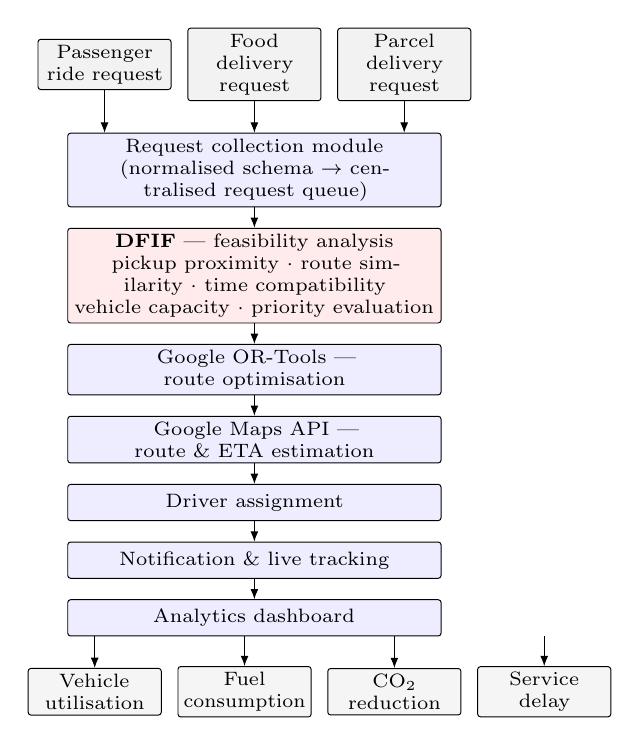
\begin{tikzpicture}[
  font=\scriptsize, node distance=2.6mm,
  bx/.style={draw,rounded corners=1pt,align=center,inner sep=2pt,
             minimum height=4.6mm,line width=0.35pt},
  src/.style={bx,fill=black!5,text width=15.5mm},
  st/.style={bx,fill=blue!7,text width=46mm},
  dfif/.style={bx,fill=red!8,text width=46mm},
  outb/.style={bx,fill=black!4,text width=15.5mm},
  ar/.style={-{Latex[length=1.3mm,width=1mm]},line width=0.35pt}]
\node[src] (r1) {Passenger\\ride request};
\node[src,right=2mm of r1] (r2) {Food delivery\\request};
\node[src,right=2mm of r2] (r3) {Parcel delivery\\request};
\node[st,below=4mm of r2] (rc) {Request collection module\\
  \scriptsize(normalised schema $\rightarrow$ centralised request queue)};
\node[dfif,below=of rc] (df) {\textbf{DFIF} --- feasibility analysis\\
  \scriptsize pickup proximity $\cdot$ route similarity $\cdot$ time
  compatibility\\ \scriptsize vehicle capacity $\cdot$ priority evaluation};
\node[st,below=of df] (ro) {Google OR-Tools --- route optimisation};
\node[st,below=of ro] (gm) {Google Maps API --- route \& ETA estimation};
\node[st,below=of gm] (da) {Driver assignment};
\node[st,below=of da] (nt) {Notification \& live tracking};
\node[st,below=of nt] (ad) {Analytics dashboard};
\node[outb,below left=4mm and -12mm of ad] (o1) {Vehicle\\utilisation};
\node[outb,right=2mm of o1] (o2) {Fuel\\consumption};
\node[outb,right=2mm of o2] (o3) {CO\textsubscript{2}\\reduction};
\node[outb,right=2mm of o3] (o4) {Service\\delay};
\foreach \s in {r1,r2,r3} \draw[ar] (\s) -- (\s |- rc.north);
\draw[ar] (rc) -- (df); \draw[ar] (df) -- (ro); \draw[ar] (ro) -- (gm);
\draw[ar] (gm) -- (da); \draw[ar] (da) -- (nt); \draw[ar] (nt) -- (ad);
\foreach \t in {o1,o2,o3,o4} \draw[ar] (ad.south -| \t) -- (\t);
\end{tikzpicture}
\caption{Architecture of the proposed AI-powered unified mobility and delivery
system.}
\label{fig:arch}
\end{figure}

\textbf{Design rationale.} The stage ordering is deliberate. Routing first
and batching opportunistically afterwards is rejected for three reasons.
Feasibility computed after routes are fixed can only accept or reject batches
that routing happened to construct, rather than searching the pending pool for
the best available one. Running the full solver over every candidate pairing,
most of which are not genuinely compatible, wastes time a cheap pre-filter
avoids. And because time-window tolerance differs sharply by service type, a
route-first approach can yield a technically shortest route that violates a
food order's window---an error the per-type tolerance in~(4) prevents
upstream. Consistent with this fail-closed policy, a request that cannot be
confidently batched is served independently on the single-service path rather
than forced into a poor match; Section~\ref{sec:props} gives this a formal
worst-case bound.

\textbf{Data handling and scalability.} Location data is retained only long
enough to complete and audit a trip, then aggregated into anonymised
statistics. Compatibility search is scoped to a geographically bounded
candidate window around each new request, so cost grows with local request
density rather than city-wide volume---the assumption formalised in~(13).
Under high load the routing and assignment modules fall back to a
proximity-only heuristic rather than stalling on an optimal solve.

\subsection{Dynamic Feasibility Intelligence Framework}
\label{sec:score}
Given a candidate pair $(i,j)$ drawn from the pending pool, the DFIF forms
the compatibility score
\begin{equation}
CS(i,j)=\alpha_1 P(i,j)+\alpha_2 R(i,j)+\alpha_3 T(i,j)
        +\alpha_4 V(i,j)+\alpha_5 Q(i,j)
\end{equation}
where $P(i,j)$ is a normalised pickup-proximity score, $R(i,j)$ a
route-similarity score, $T(i,j)$ a time-window overlap score, $V(i,j)$ a
vehicle-capacity feasibility indicator, $Q(i,j)$ a priority-compatibility
score, and $\alpha_1,\dots,\alpha_5$ are weighting coefficients satisfying
$\sum_{k=1}^{5}\alpha_k=1$, tuned so that time-window overlap is weighted
more heavily for food-delivery requests than for passenger or parcel requests.
A pair is considered feasible for batching when
\begin{equation}
CS(i,j)\ \ge\ \tau,
\end{equation}
where $\tau$ is a feasibility threshold calibrated during system tuning.

The time-window overlap term is computed as
\begin{equation}
T(i,j)=\max\!\left(0,\ 1-\frac{|t_i-t_j|}{W_{\text{type}}}\right)
\end{equation}
where $t_i$ and $t_j$ are the requested service times and $W_{\text{type}}$ is
a service-type-specific tolerance window---smaller for food delivery, larger
for parcel delivery---so that the same absolute time gap between two requests
produces a lower compatibility score when at least one of the requests is a
food order. Capacity enters as a binary admissibility flag rather than a graded score,
because it is a hard constraint: once a batch overruns the seating or cargo volume available, no degree of
proximity or timing agreement can rescue it,
\begin{equation}
V(i,j)=\begin{cases}
1, & cap(i)+cap(j)\le Cap_{\max},\\
0, & \text{otherwise},
\end{cases}
\end{equation}
where $cap(i)$ and $cap(j)$ denote the seating or cargo capacity required by
requests $i$ and $j$, and $Cap_{\max}$ is the capacity of the candidate
vehicle. Any pair for which $V(i,j)=0$ is excluded from batching regardless of
its score on the other four criteria. Finally, the priority term
\begin{equation}
Q(i,j)=1-\frac{|pri(i)-pri(j)|}{pri_{\max}}
\end{equation}
captures how far apart the two requests sit on the service-level scale, so
that batching throughput is not bought by routinely postponing urgent work: pairs separated by a wide priority gap are penalised even where proximity and
timing would otherwise recommend them.

\subsection{Feasibility-First Routing and Driver Assignment}
For an admitted batch $B=\{r_1,\dots,r_k\}$, the routing stage searches for
the pickup and drop-off ordering $\pi$ that minimises
\begin{equation}
\min_\pi\ \bigl[\beta_1 d(\pi)+\beta_2 t(\pi)+\beta_3\,\mathit{Idle}(\pi)\bigr]
\end{equation}
subject to vehicle-capacity constraints and the per-request time windows
established in~(4), where $d(\pi)$ is total travel distance under ordering
$\pi$, $t(\pi)$ is total travel time, $\mathit{Idle}(\pi)$ is expected vehicle
idle time, and $\beta_1,\beta_2,\beta_3$ are tunable coefficients reflecting
the platform's relative priority on distance, time, and idle-time
minimisation. For an optimised route $\rho$ and a candidate driver $d$, the
assignment module computes an assignment cost
\begin{equation}
\mathit{Cost}(d,\rho)=\gamma_1 \mathit{dist}(d,\rho)
 +\gamma_2 \mathit{ETA}(d,\rho)+\gamma_3 \mathit{CapMismatch}(d,\rho)
\end{equation}
where $\mathit{dist}(d,\rho)$ is the driver's distance to the route's first
pickup, $\mathit{ETA}(d,\rho)$ is the estimated time to reach it,
$\mathit{CapMismatch}(d,\rho)$ penalises assigning a vehicle whose capacity
poorly matches the batch's requirements, and $\gamma_1,\gamma_2,\gamma_3$ are
weighting coefficients. The system selects
\begin{equation}
d^{*}=\argmin_{d\in D_{\text{available}}}\mathit{Cost}(d,\rho)
\end{equation}
among the set of currently available drivers $D_{\text{available}}$.

\subsection{Theoretical Analysis}
\label{sec:props}

\textbf{Boundedness.} The four graded terms lie in $[0,1]$ by construction,
$V$ is binary, and the weights are non-negative and sum to one, so~(2) is a
convex combination of quantities drawn from $[0,1]$; hence
\begin{equation}
CS(i,j)\in[0,1]\quad\forall i,j,
\end{equation}
The practical consequence is that $\tau$ in~(3) carries the same meaning for
any two request pairs, however unlike, and survives the addition of further
criteria without rescaling.

\textbf{Lipschitz sensitivity of the time term.} From~(4), for fixed $t_j$ the
function $t_i\mapsto T(i,j)$ is piecewise-linear with slope of magnitude
$1/W_{\text{type}}$ wherever $T(i,j)>0$, so
\begin{equation}
|T(i,j)-T(i',j)|\ \le\ \frac{1}{W_{\text{type}}}\,|t_i-t_{i'}|,
\end{equation}
and $T(\cdot,j)$ is $\tfrac{1}{W_{\text{type}}}$-Lipschitz in the request
time. With $W_{\text{type}}$ set narrower for meals than for packages, an
identical timing offset costs a food pairing strictly more score than it costs
a parcel pairing. The informal statement that meals are the time-critical case
therefore becomes an inequality that can be read straight off the deployed
tolerance constants, and it underwrites the uneven delay result analysed in
Section~\ref{sec:results}.

\begin{proposition}[Fail-closed suboptimality bound]
\label{prop:fc}
Write $C_0(r)$ for the cost of dispatching request $r$ on its own under the
single-service baseline, and $C_{\mathrm{DFIF}}$ for the total cost the system
actually incurs over a pool $\mathcal{R}$. Provided every request that clears
no partner under~(3) falls back to the baseline path,
\begin{equation}
C_{\mathrm{DFIF}}\ \le\ \sum_{r\in\mathcal{R}}C_0(r).
\end{equation}
\end{proposition}

\begin{proof}[Proof sketch]
Split $\mathcal{R}$ into a batched part $\mathcal{R}_B$ and its complement
$\mathcal{R}_U$. The fail-closed rule charges each $r\in\mathcal{R}_U$ exactly
$C_0(r)$. Any $r\in\mathcal{R}_B$ entered a batch only after~(7)--(8) returned
a route and driver whose share of the realised cost is bounded above by the
cost of serving $r$ alone, since serving $r$ alone is itself a feasible point
of~(7) and the solver's optimum can be no worse than any feasible point.
Adding the two parts yields the stated bound.
\end{proof}

\textbf{Compatibility graph and complexity.} The batching decision can be
posed as a graph problem. Take $G=(\mathcal{R},E)$ over the pending pool, admitting the edge $(i,j)$
exactly when $CS(i,j)\ge\tau$ and $V(i,j)=1$. Choosing the best set of
mutually compatible batches then amounts to capacity-constrained
maximum-weight clique packing on $G$, each clique weighted by the distance and
time it would save under~(7)---NP-hard in the general case.
Rather than solving this exactly citywide, the bounded candidate window
restricts each request to at most $k$ neighbours, so scoring one request costs
$O(k)$ evaluations of~(2) instead of $O(|\mathcal{R}|)$, and the full pool
costs
\begin{equation}
O(|\mathcal{R}|\cdot k)\quad\text{instead of}\quad O(|\mathcal{R}|^2),
\end{equation}
with $k\ll|\mathcal{R}|$ under the density assumption stated in
Section~\ref{sec:limits}. The DFIF does not avoid the underlying NP-hardness
of joint batch selection---neither does the AVIS mixed-integer
formulation~\cite{zhang2022}, nor the capacitated vehicle-routing problem with
time windows that OR-Tools solves---but what it does change is the graph on
which that hardness is paid, shrinking it from citywide to local and
bounded-degree before the costlier routing stage in~(7) runs.

\textbf{Driver assignment as a linear assignment problem.} As written,~(9) is a greedy per-batch $\argmin$ applied separately to each
newly optimised route. Its cost is $O(|D_{\text{available}}|)$ per assignment,
but it offers no guarantee of a globally optimal pairing once several routes
and several drivers are settled within one dispatch cycle. The globally optimal version is
the classical linear assignment problem: with $m$ routes awaiting drivers and $n$ drivers free, assemble
$\mathbf{C}\in\mathbb{R}^{m\times n}$ via
$\mathbf{C}_{\rho,d}=\mathit{Cost}(d,\rho)$ from~(8), then solve
\begin{equation}
\pi^{*}=\argmin_{\pi\in\Pi}\sum_{\rho}\mathbf{C}_{\rho,\pi(\rho)},
\end{equation}
where $\Pi$ is the set of one-to-one matchings between routes and drivers.
Equation~(14) is solvable exactly by the Hungarian
algorithm~\cite{kuhn1955} in $O(\max(m,n)^3)$, or nearer $O(mn\log n)$ with
modern shortest-augmenting-path implementations. The greedy rule~(9) is used in the
reference implementation for its low-latency budget;~(14) bounds the
assignment quality that simplification may forgo.

\subsection{Adaptive Coefficient Learning}
\label{sec:learn}
Sections~\ref{sec:score}--\ref{sec:props} establish the DFIF's behaviour
under a fixed weight vector $\alpha=(\alpha_1,\dots,\alpha_5)$. Treating
$\alpha$ as hand-tuned is what separates a rule-based filter from a learning
system; closing that gap is the framework's artificial-intelligence
contribution.

\textbf{Simplex-constrained parameterisation.} Direct gradient updates on
$\alpha$ risk violating $\sum_k\alpha_k=1$ and $\alpha_k\ge0$. To avoid
re-projecting onto the simplex each iteration, $\alpha$ is generated from an
unconstrained latent vector $\theta=(\theta_1,\dots,\theta_5)$ by softmax:
\begin{equation}
\alpha_k=\frac{\exp(\theta_k)}{\sum_{m=1}^{5}\exp(\theta_m)},
\qquad k=1,\dots,5.
\end{equation}
Because a softmax output always lies on the probability simplex,~(15)
automatically satisfies the constraints under which the boundedness property
in~(10) was proven, for any $\theta\in\mathbb{R}^5$, so learning can proceed
as unconstrained optimisation over $\theta$.

\textbf{Outcome-driven loss.} Write $\ell(i,j)\in\{0,1\}$ for the retrospective verdict on a batch built
from $i$ and $j$: one when every window was met and the dashboard recorded a
positive distance and fuel saving against independent dispatch, zero
otherwise. The per-pair loss is the binary cross-entropy between the DFIF's
predicted compatibility and the observed outcome,
\begin{equation}
\mathcal{L}(\theta)=-\bigl[\ell(i,j)\log CS(i,j)
 +\bigl(1-\ell(i,j)\bigr)\log\bigl(1-CS(i,j)\bigr)\bigr].
\end{equation}

\textbf{Gradient update.} Since $CS(i,j)$ is linear in $\alpha$ by~(2), its
gradient with respect to each softmax weight is simply the corresponding
feature value,
\begin{equation}
\frac{\partial CS(i,j)}{\partial\alpha_k}=F_k(i,j),
\qquad F_k\in\{P,R,T,V,Q\},
\end{equation}
and the softmax Jacobian gives, for every pair $(k,m)$,
\begin{equation}
\frac{\partial\alpha_k}{\partial\theta_m}=\alpha_k(\delta_{km}-\alpha_m),
\end{equation}
with $\delta_{km}$ the Kronecker delta. Combining~(16)--(18) by the chain rule
gives the full per-parameter gradient
$\partial\mathcal{L}/\partial\theta_m=
\sum_k(\partial\mathcal{L}/\partial CS)(\partial CS/\partial\alpha_k)
(\partial\alpha_k/\partial\theta_m)$, and the online update rule
\begin{equation}
\theta_m\leftarrow\theta_m-\eta\,
\frac{\partial\mathcal{L}(\theta)}{\partial\theta_m},\qquad m=1,\dots,5,
\end{equation}
with learning rate $\eta>0$, applied after each completed trip is scored.
This is the mechanism by which the weighting coefficients can be calibrated
against real operational data rather than fixed a priori.

\textbf{Threshold adaptation.} The threshold $\tau$ in~(3) is tunable by the
same signal. Treating $\tau$ as the operating point of a binary classifier
over $CS(i,j)$ against $\ell(i,j)$, the expected utility is
\begin{equation}
\mathbb{E}[U(\tau)]=\Pr\bigl(CS\ge\tau\mid\ell=1\bigr)u^{+}
 -\Pr\bigl(CS\ge\tau\mid\ell=0\bigr)u^{-},
\end{equation}
where $u^{+}$ and $u^{-}$ are the realised utility of a correctly and an
incorrectly accepted batch, and $\tau^{*}=\argmax_\tau\mathbb{E}[U(\tau)]$
moves the threshold to the empirically optimal operating point.

\textbf{Implemented extensions and their validation status.}
\label{sec:algs}
Equations~(2)--(20) specify the DFIF as closed-form relations. Three
procedures realise them end to end in the implementation---incremental
compatibility-graph construction under the bounded-neighbourhood assumption
of~(13), an online softmax-weight update fusing~(15)--(19) into one
adaptive-moment step, and a latency-budgeted assignment rule that also
recalibrates $\tau$ via~(20)---and are given in Algorithm~1. Per-call cost is
$O(k)$ per request, $O(1)$ per completed trip, and $O(\max(m,n)^3)$ exact or
$O(|D|)$ fallback for assignment, adding no asymptotic overhead beyond~(13).

\textbf{These three procedures were not exercised in the pilot deployment
reported in Section~\ref{sec:results}.} Their empirical evaluation---alongside
the larger-sample statistical testing already identified in
Section~\ref{sec:limits}---is left for the multi-area trial planned as the
next step. The results reported below evaluate the base DFIF pipeline
described in Sections~\ref{sec:score}--\ref{sec:props}.

\subsection{Provenance of the Formulation}
Because the framework assembles standard mathematical constructions alongside
relations specific to this work, it is worth stating plainly which is which.
Equations~(2), (3), (10), (12) and~(13) are particular to this paper: the
five-criterion compatibility score and its admission rule, the boundedness
result, the fail-closed bound of Proposition~\ref{prop:fc}, and the complexity
statement under a bounded candidate neighbourhood. The remainder instantiate
established forms rather than introduce new mathematics. Equations~(4)
and~(6) are normalised-difference similarity kernels, with the service-type
tolerance $W_{\text{type}}$ the element contributed here; (5) is the capacity
indicator conventional in capacitated vehicle routing; (7) and~(8) are
weighted-sum scalarisations of the routing and assignment objectives in the
form usual for pickup-and-delivery problems with time windows; and~(14) is the
classical linear assignment problem, solved by the Hungarian
method~\cite{kuhn1955}. Equations~(15), (16), (18) and~(19) are respectively
the softmax parameterisation, the binary cross-entropy loss, the softmax
Jacobian, and the stochastic-gradient update---all standard in machine
learning, applied here to the weight vector $\alpha$---while~(20) expresses
the expected utility of a decision threshold in the usual
receiver-operating-characteristic form. Equation~(1) is an evaluation device
defined in this paper for Table~\ref{tab:related} and is not claimed as a
contribution. The novelty therefore lies not in the individual constructions
but in their composition into a feasibility-first layer spanning three service
types, and in the properties established in Section~\ref{sec:props}.

\begin{figure}[t]
\footnotesize
\hrule height 0.8pt \vspace{2pt}
\noindent\textbf{Algorithm 1\ \ DFIF operational pipeline}
\vspace{2pt}\hrule height 0.4pt \vspace{3pt}
\noindent\textbf{A. Bounded-neighbourhood graph construction (per request $r$)}

\vspace{1pt}\noindent
\hspace*{0.6em}1: $\mathit{cands}\leftarrow\textsc{GeoKNN}(r,\mathcal{R},k)$
 \hfill $O(k)$, not $O(|\mathcal{R}|)$\\
\hspace*{0.6em}2: \textbf{for} $c\in\mathit{cands}$: \textbf{if} $V(r,c)=0$
 \textbf{continue} \hfill prune on (5) first\\
\hspace*{0.6em}3: \hspace*{0.8em}$\alpha\leftarrow\mathrm{softmax}(\theta)$;
 evaluate $CS(r,c)$ \hfill (15), (2), (4), (6)\\
\hspace*{0.6em}4: \hspace*{0.8em}\textbf{if} $CS\ge\tau$:
 $E\leftarrow E\cup\{(r,c,CS)\}$ \hfill (3)\\
\hspace*{0.6em}5: insert $r$ into spatial index; take connected component\\
\hspace*{0.6em}6: \textbf{if} $|\mathrm{comp}|\ge2$:
 $B\leftarrow B\cup\textsc{CliquePack}(\mathrm{comp})$
 \hfill bounded by $|\mathrm{comp}|$

\vspace{3pt}\noindent\textbf{B. Online softmax weight update (per completed trip)}

\vspace{1pt}\noindent
\hspace*{0.6em}7: $\alpha\leftarrow\mathrm{softmax}(\theta)$;
 $CS\leftarrow\sum_k\alpha_k F_k$ \hfill (15), (2)\\
\hspace*{0.6em}8: $\mathcal{L}\leftarrow
 -[\ell\log CS+(1-\ell)\log(1-CS)]$ \hfill (16)\\
\hspace*{0.6em}9: $g_k\leftarrow
 \bigl(-\tfrac{\ell}{CS}+\tfrac{1-\ell}{1-CS}\bigr)
 \alpha_k\bigl(F_k-\sum_m\alpha_m F_m\bigr)$ \hfill (17), (18) fused\\
\hspace*{0.4em}10: clip $g_k$; adaptive-moment step on $\theta$ \hfill (19)

\vspace{3pt}\noindent\textbf{C. Latency-budgeted assignment (per dispatch cycle)}

\vspace{1pt}\noindent
\hspace*{0.4em}11: build $\mathbf{C}_{\rho,d}$ from (8)\\
\hspace*{0.4em}12: \textbf{if} estimated Hungarian cost $\le T_{\max}$:
 $\pi^{*}\leftarrow$ Hungarian$(\mathbf{C})$ \hfill (14)\\
\hspace*{0.4em}13: \textbf{else} order $\rho$ by ascending $W_{\text{type}}$,
 apply (9) \hfill (11) fallback\\
\hspace*{0.4em}14: every $N$ completions:
 $\tau^{*}\leftarrow\argmax_\tau\mathbb{E}[U(\tau)]$ \hfill (20)

\vspace{2pt}\hrule height 0.8pt
\end{figure}

\section{Experimental Setup}

\subsection{Test Environment}
Validation used a controlled deployment over a defined urban test area,
driven by generated passenger-ride, food-delivery, and parcel-delivery
requests. The Google Maps API supplied real travel-distance,
route, and travel-time data for every request rather than simulated distances.
Each entry recorded its origin, destination, requested window, and payload
type, matching the shared schema of Section~\ref{sec:method}.

\subsection{Baseline}
The comparison baseline is a traditional, non-unified dispatch configuration
that assigns and routes each service type independently, with no cross-service
batching. It operates on the same request set and the same mapping data as the
DFIF configuration, so the two differ only in whether feasibility-first
batching is applied.

\subsection{Evaluation Metrics}
Metrics were defined ahead of data collection so that the comparison is
measured consistently; Table~\ref{tab:metrics} states each definition. Taken
with the compatibility-score distribution, they indicate whether
feasibility-first batching improved operational efficiency without degrading
service-level quality for any individual request.

\begin{table}[t]
\caption{Evaluation metrics and definitions}
\label{tab:metrics}
\centering
\footnotesize
\setlength{\tabcolsep}{4pt}
\begin{tabular}{@{}p{0.27\columnwidth}p{0.63\columnwidth}@{}}
\toprule
Metric & Definition \\
\midrule
Vehicle utilisation rate &
Proportion of a driver's active shift spent transporting an active
request---passenger, food, or parcel---rather than idle or repositioning. \\
Travel-distance reduction &
Percentage difference between total vehicle-kilometres under DFIF-based
batching and under the independent-dispatch baseline for an equivalent
request set. \\
Average delay &
Mean difference between a request's actual service time and its originally
requested time window. \\
Estimated CO\textsubscript{2} &
Derived from total distance travelled using a standard per-kilometre
emissions factor for the vehicle types in the test fleet. \\
\bottomrule
\end{tabular}
\end{table}

\section{Results and Discussion}
\label{sec:results}

\subsection{Pilot Deployment}
Deployment covered a pilot set of requests drawn from all three
categories---passenger rides, food orders, and parcel drops---inside a bounded
urban area, with feasibility scoring, routing, and driver assignment wired
together end to end. No distances were synthesised: every request's distance,
travel time, and route came from the Google Maps API. Across the pilot window, 43 requests entered the platform through three live
provider integrations: 12 from Rapido (27.9\%), 17 from Swiggy (39.5\%), and
14 from Delhivery (32.6\%). Arrivals peaked at 17:00, and mean end-to-end
processing took 327.9 seconds per request. Thirty of the 43 reached
completion---a 69.8\% completion rate---and the DFIF assembled 3 feasible
batches, turning away 2 candidate pairs that fell below the threshold. The
scale here supports a directional reading only. This is not a powered trial:
$n=43$ leaves no room for the subgroup or significance analysis flagged in
Section~\ref{sec:limits}, and a larger trial is the intended next step.

\subsection{Compatibility Score Distribution}
Fig.~\ref{fig:compat} shows the distribution of DFIF compatibility scores
$CS(i,j)$ from~(2) computed across the pending request pairs in the pilot
dataset. In line with the density assumption recorded in
Section~\ref{sec:limits}, the mass of the distribution sat comfortably above
the admission threshold $\tau$: most pairs fell in the 70--95\% range, and
the modal band was 80--85\%. Two independent readings agree. The deployed explainability dashboard logged
an average compatibility score of 77.1\% alongside an overall XAI score of
87\%, and the engine's live pending queue held a 73.7\% mean across the
standing request pool. This shape indicates that, at the request density present in the test area,
genuinely compatible pairings were common rather than rare---the precondition
for the efficiency gains below. A distribution skewed toward low scores would
instead have indicated density too sparse for feasibility-first batching to
add value, a scenario the pilot was designed to detect rather than assume
away and one retained as a limitation in Section~\ref{sec:limits}.

\begin{figure}[t]
\centering
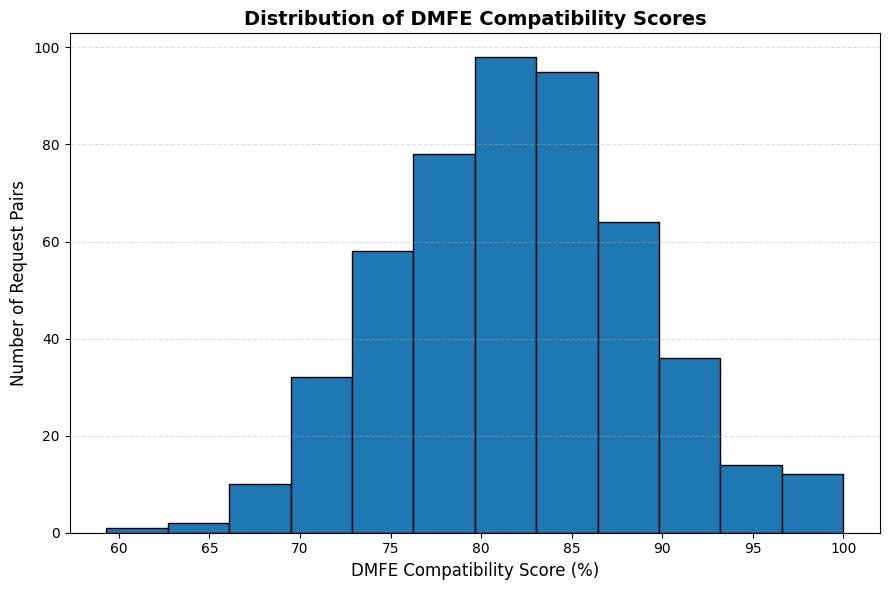
\includegraphics[width=\columnwidth]{fig_compat_orig.png}
\caption{Distribution of DFIF compatibility scores across pending request
pairs.}
\label{fig:compat}
\end{figure}

\subsection{Route Optimisation and Overall Performance}
Fig.~\ref{fig:perf} sets four quantities---distance, fuel, mean delay, and
estimated CO\textsubscript{2}---side by side for the same pilot fleet run
first without feasibility-first batching and then with it, the latter also
carrying OR-Tools optimisation under~(7). Over the pilot period, distance travelled dropped from 320~km to 250~km,
fuel drawn from 38~L to 30~L, mean per-request delay from 12~minutes to
7~minutes, and estimated CO\textsubscript{2} from 80~kg to 63~kg---reductions
of 21.9\%, 21.1\%, 41.7\%, and 21.3\% in that order.

\begin{figure}[t]
\centering
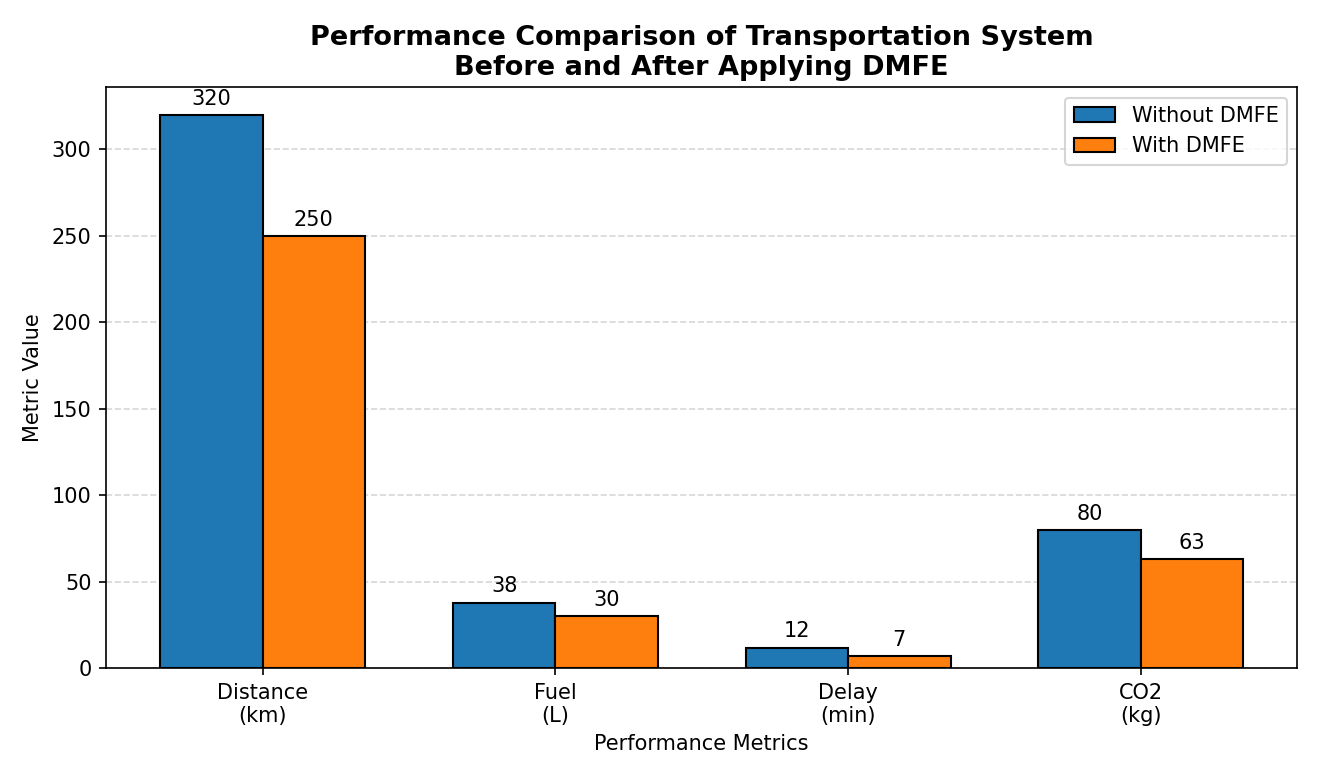
\includegraphics[width=\columnwidth]{fig_perf_orig.png}
\caption{Performance comparison of the transportation system before and after
applying DFIF-based batching.}
\label{fig:perf}
\end{figure}

The largest single gain, 41.7\%, landed on delay, which is what the
sensitivity argument in~(11) and the design intent behind~(4) jointly imply:
since admission weighed each request's own tolerance window instead of
treating every request as equally patient, fewer requests ended up queued
behind an ill-matched partner. The remaining three moved almost together---
21.9\%, 21.1\%, and 21.3\%---which is unsurprising given that distance,
fuel, and emissions are near-linear in vehicle-kilometres, so cutting the
first cuts the other two by roughly the same proportion. Over the wider deployment window---distinct from the 43-request pilot
period above---the platform recorded 2,320 shared trips, a cumulative fuel
saving of 611.3~L, and a cumulative CO\textsubscript{2} reduction of
1,406.01~kg. The analytics dashboard reported an overall AI confidence
(system intelligence) score of 98.4\% and a batch success rate of 92.1\%
across the same window.

\subsection{Comparative Discussion}
These figures were compared against the direction, though not the magnitude,
of results published for joint-optimisation systems. AVIS reported that
optimising rides and parcels together cut redundant vehicle movement against
handling the two categories apart~\cite{zhang2022}, and hybrid routing studies
record double-digit distance and delay reductions once a dynamic,
constraint-aware layer displaces independent dispatch~\cite{lu,liu2025}. What
those single-service systems would not anticipate is the gap between the delay
figure and the distance-linked ones---41.7\% against roughly 21.1--21.9\%---
because none of them varies timing tolerance by category as $T(i,j)$ does
in~(4). The pilot reproduced that gap closely, delay moving at near twice the
rate of the distance-linked measures, which points to the per-type timing
weight rather than route optimisation as the dominant source. Establishing
that attribution properly needs an ablation---the same pipeline run with a
single undifferentiated timing term---which this pilot did not cover and which
is recorded as future evaluation work.

The asymmetry was predicted rather than observed post hoc. Because
$T(\cdot,j)$ is $1/W_{\text{type}}$-Lipschitz by~(11) and $W_{\text{type}}$
is tighter for food orders, $CS(i,j)$ is mathematically more sensitive to time
misalignment for food-delivery pairs, so batching was expected a priori to
correct delay more aggressively than distance---which carries no
service-type-specific weighting in~(7) beyond the upstream feasibility gate.
The reviewed baselines~\cite{zhang2022,lu,liu2025} carry no equivalent
per-type component, and their reported gains are correspondingly closer to
uniform across metrics.

\subsection{Interpretation and Caveats}
The pilot results support the core hypothesis that feasibility-first batching
outperforms independent dispatch; even so, three caveats limit how far the
numbers should be generalised at this stage. First, the pilot ran in a single bounded test area whose request density
favoured batching, as Fig.~\ref{fig:compat} reflects; lower-density areas were
not separately tested, and by~(13) a sparser pool shrinks the candidate
neighbourhood $k$, which would lower realised compatibility scores rather than
merely reduce the evaluation sample. Second, Fig.~\ref{fig:perf} reports
aggregate totals over the pilot period, not per-request or per-service-type
breakdowns, so it cannot be said whether the gains were shared evenly across
the three categories or concentrated in one. Third, vehicle-utilisation rate
and the driver-assignment metrics---ETA accuracy and capacity-mismatch
rate---were not part of the figures this round supplied, and are left to a
subsequent cycle alongside the larger-sample statistical testing needed for
significance and the empirical validation of~(19), which requires more
completed-trip outcomes than this pilot generated.

\section{Limitations and Future Work}
\label{sec:limits}
Four limitations bound what the current design and evaluation can claim. Section~\ref{sec:results} reports a single-area pilot, not a powered
large-scale trial, so the size of the reported gains reads as an early directional signal rather
than a transferable benchmark, until retested across several areas and demand
profiles. The weighting coefficients and the admission threshold $\tau$ remain
unlearned design parameters at this stage; until~(19) has been run against
real operating data, batching behaviour should be read as provisional. Routing and assignment quality depends on third-party mapping data;
degraded or delayed Google Maps API responses would directly reduce the
reliability of both the feasibility scores and the resulting routes. The
design assumes reasonably dense, overlapping demand across all three service
types, and~(13) shows why this matters---a small candidate neighbourhood $k$
mechanically shrinks the number of pairs that can clear $\tau$---so the
benefit over independent dispatch must be evaluated separately for sparse
conditions. Finally, driver and customer acceptance of batched multi-purpose
trips has not been evaluated. Equation~(6) treats priority as a
system-assigned numeric level; how that level is set in practice---by
service-level agreement, surge pricing, or customer-selected urgency---is a
policy question outside this paper's technical scope but one that will
materially affect deployed batching behaviour.

Several directions extend naturally from the current design. How much proximity should count against timing overlap plausibly shifts with
city density and hour of day, so $\alpha_1,\dots,\alpha_5$ in~(2) and $\tau$
in~(3) ought to be fitted to observed operation rather than chosen up front.
Section~\ref{sec:learn} already casts that fitting as~(19) and~(20); what
remains is to run it on outcome data at volume, not to design it. A second
direction is congestion forecasting inside the routing module, so the system
anticipates traffic instead of consuming whatever travel-time estimate the
mapping API returns at planning time. A third is demand prediction, which
would let idle drivers be positioned ahead of a surge rather than dispatched
after it. Longer term, replacing the hand-specified cost functions
in~(7)--(8) with a learned assignment policy is attractive; comparable
policies have been demonstrated for joint matching, pricing, and
dispatching~\cite{haliem2021,manchella2022}, and~(14) supplies the
optimal-policy reference such a learner would have to match.

\section{Conclusion}
Three dispatch problems that share a road network are still solved
separately, and the cost of that separation is trips no coordinated dispatcher
would have made. This paper answered it with a feasibility-first decision
layer: a five-criterion compatibility score settled before routing or driver
selection, a formal profile covering boundedness, timing sensitivity,
worst-case suboptimality and complexity, a softmax-parameterised learning rule
for the weights, constraint-based routing, and multi-factor driver assignment,
all in one pipeline spanning rides, meals, and parcels. Pilot evidence over 43
requests showed delay falling 41.7\% against roughly 21\% for the
distance-linked measures---the uneven split that~(11) anticipates, not a
uniform gain. The binding limitation is scale: one area, 43 requests, no
statistical power, and a learning rule specified but not yet trained. The next
step is a multi-area trial large enough to carry the utilisation and
assignment metrics this round omitted and to exercise~(19) on real
completed-trip outcomes.

\balance
\begin{thebibliography}{12}

\bibitem{santi2014}
P.~Santi, G.~Resta, M.~Szell, S.~Sobolevsky, S.~H. Strogatz, and C.~Ratti,
``Quantifying the benefits of vehicle pooling with shareability networks,''
\emph{Proc. Nat. Acad. Sci. USA}, vol.~111, no.~37, pp.~13290--13294, 2014,
doi: 10.1073/pnas.1403657111.

\bibitem{seng2023}
K.~P. Seng, L.-M. Ang, E.~Ngharamike, and E.~Peter, ``Ridesharing and
crowdsourcing for smart cities: Technologies, paradigms and use cases,''
\emph{IEEE Access}, vol.~11, pp.~18038--18081, 2023,
doi: 10.1109/ACCESS.2023.3243264.

\bibitem{zhang2022}
S.~Zhang, C.~Markos, and J.~J.~Q. Yu, ``Autonomous vehicle intelligent system:
Joint ride-sharing and parcel delivery strategy,'' \emph{IEEE Trans. Intell.
Transp. Syst.}, vol.~23, no.~10, pp.~17457--17472, Oct. 2022.

\bibitem{haliem2021}
M.~Haliem, G.~Mani, V.~Aggarwal, and B.~Bhargava, ``A distributed model-free
ride-sharing approach for joint matching, pricing, and dispatching using deep
reinforcement learning,'' \emph{IEEE Trans. Intell. Transp. Syst.}, vol.~22,
no.~12, pp.~7933--7951, Dec. 2021.

\bibitem{manchella2022}
K.~Manchella, M.~Haliem, V.~Aggarwal, and B.~Bhargava, ``PassGoodPool: Joint
passengers and goods fleet management with reinforcement learning aided
pricing, matching, and route planning,'' \emph{IEEE Trans. Intell. Transp.
Syst.}, vol.~23, no.~11, pp.~20854--20868, Nov. 2022.

\bibitem{hong2019}
H.~Hong, X.~Li, D.~He, Y.~Zhang, and M.~Wang, ``Crowdsourcing incentives for
multi-hop urban parcel delivery network,'' \emph{IEEE Access}, vol.~7,
pp.~26255--26267, 2019.

\bibitem{berahhou}
A.~Berahhou and Y.~Benadada, ``Dynamic vehicle routing problem:
State-of-the-art review.''
\textbf{[UNVERIFIED --- COMPLETE BEFORE SUBMISSION: venue, year, DOI]}

\bibitem{chen2022}
J.-F. Chen, T.-H. Chang, and Y.-H. Chang, ``An imitation learning-enhanced
iterated matching algorithm for on-demand food delivery,'' \emph{IEEE Trans.
Intell. Transp. Syst.}, vol.~23, no.~11, pp.~21803--21817, Nov. 2022.

\bibitem{lu}
Y.~Lu \emph{et al.}, ``Collaborative hybrid delivery framework combining
riders and drones.''
\textbf{[UNVERIFIED --- COMPLETE BEFORE SUBMISSION: venue, year, DOI]}

\bibitem{liu2025}
Z.~Liu, X.~Zuo, M.~C. Zhou, B.~Jia, and C.~Xin, ``Meal delivery routing problem
with a hybrid fleet of riders and autonomous vehicles under dynamic
environment,'' \emph{IEEE Trans. Autom. Sci. Eng.}, vol.~22,
pp.~11642--11655, 2025, doi: 10.1109/TASE.2025.3534143.

\bibitem{ortools}
L.~Perron and V.~Furnon, ``OR-Tools,'' Google. [Online]. Available:
\url{https://developers.google.com/optimization/}

\bibitem{kuhn1955}
H.~W. Kuhn, ``The Hungarian method for the assignment problem,'' \emph{Naval
Res. Logist. Quart.}, vol.~2, no.~1--2, pp.~83--97, 1955,
doi: 10.1002/nav.3800020109.

\end{thebibliography}

\end{document}
